\pdfoutput=1

\documentclass[11pt]{article}

% Remove the "review" option to generate the final version.
\usepackage{EMNLP2023}
% \usepackage[review]{EMNLP2023}

% Standard package includes
\usepackage{times}                            % font style
\usepackage{latexsym}                         % for additional symbols
\usepackage[T1]{fontenc}
\usepackage[utf8]{inputenc} 
\usepackage{microtype}                        % better types
\usepackage{inconsolata}                      % truetype font style
\usepackage{booktabs}                         % better-looking tables
\usepackage[raggedrightboxes]{ragged2e}       % better table alignment
\usepackage{subfiles}                         % file management
\usepackage{longtable}                        % multi-column tables
\usepackage{amsmath}                          % math symbols and equations
\usepackage{graphicx}                         % inserting images


\title{calamanCy: A Tagalog Natural Language Processing Toolkit}

\author{Lester James V. Miranda \\
  ExplosionAI GmbH \\
  \texttt{lj@explosion.ai}}

\begin{document}
\maketitle
\begin{abstract}
  We introduce calamanCy, an open-source toolkit for constructing natural language processing (NLP) pipelines for Tagalog.
  It is built on top of spaCy, enabling easy experimentation and integration with other frameworks.  
  calamanCy addresses the development gap by providing a consistent API for building NLP applications and offering general-purpose multitask models with out-of-the-box support for dependency parsing, part-of-speech (POS) tagging, and named entity recognition (NER).
  calamanCy aims to accelerate the progress of Tagalog NLP by consolidating disjointed resources in a unified framework.
  The calamanCy toolkit can be found on Github: \url{https://github.com/ljvmiranda921/calamanCy}.
\end{abstract}

\section{Introduction}

Tagalog is a low-resource language from the Austronesian family with over 76 million speakers in the Philippines \citep{Lewis2009EthnologueL}.
Despite its speaker population, few resources exist for the language \citep{Cruz2021ImprovingLL}. 
For example, Universal Dependencies (UD) treebanks for Tagalog are tiny ($\ll$ 20k words) \citep{Samson2018TRG,Aquino2020ParsingIT}, 
while domain-specific corpora are sparse \citep{Cabasag2016HatespeechIP,Livelo2018IntelligentDI}. 
In addition, Tagalog language models (LMs) \citep{Cruz2021ImprovingLL,Jiang2021PretrainedLM} are few while most multilingual LMs \citep{Conneau2019UnsupervisedCR,Devlin2019BERTPO} underrepresent the language.
Thus, consolidating these disjointed resources in a coherent framework is still an open problem.
The lack of such framework hampers model development, experimental workflows, and the overall advancement of Tagalog NLP.

To address this problem, we introduce calamanCy,\footnote[1]{
  The name ``calamanCy'' came from \textit{kalamansi}, a citrus fruit native to the Philippines.}
an open-source toolkit for Tagalog NLP. 
It is built on top of spaCy \citep{Honnibal2020Spacy} and offers end-to-end pipelines for NLP tasks such as dependency parsing, parts-of-speech (POS) tagging, and named entity recognition (NER). 
calamanCy also provides models of different sizes to fit any performance or accuracy requirements.
This work has two main contributions: (1) an open-source toolkit containing general-purpose multitask pipelines with out-of-the box support for common NLP tasks, and (2) structured benchmarks that evaluate on several Tagalog core NLP tasks.

\subfile{tables/entity_types}


\section{Related Work}

\paragraph*{Open-source toolkits for NLP}
There has been a growing body of work in the development of NLP toolkits in recent years. 
For languages, these toolkits include DaCy for Danish \citep{Enevoldsen2021DaCyAU} and HuSpaCy for Hungarian \citep{Orosz2022HuSpaCyAI}.
For domain-specific data, there is medspaCy for clinical text \citep{Eyre2021LaunchingIC} and scispaCy for scientific documents \citep{Neumann2019ScispaCyFA}.
These tools employ spaCy \citep{Honnibal2020Spacy}, an industrial-strength open-source software for natural language processing.
Using spaCy as a foundation is an optimal choice given its popularity and tight integration with other frameworks such as HuggingFace \citep{Wolf2019HuggingFacesTS}.
However, no tool exists for Tagalog until now.
In this paper, we will showcase how calamanCy provides similar capabilities to DaCy and HuSpaCy using Tagalog resources.

\paragraph*{Evaluations on Tagalog NLP Tasks} 
Structured evaluations for core NLP tasks, such as dependency parsing, POS tagging, and NER, are sparse.
However, we have access to a reasonable amount of data to conduct comprehensive benchmarks.
For example, TLUnified \citep{Cruz2021ImprovingLL} is a pretraining corpus that combines news reports \citep{Cruz2020ExploitingNA}, a preprocessed version of CommonCrawl \citep{OrtizSuarez2019AsynchronousPF}, and several other datasets.
However, it was evaluated on domain-specific applications that may not easily transfer to more general tasks.
For dependency parsing and POS tagging, we have Universal Dependencies treebanks such as TRG \citep{Samson2018TRG} and Ugnayan \citep{Aquino2020ParsingIT}.
This paper will fill the evaluation gap by providing structured benchmarks on these core tasks.

\section{Implementation}

The best way to use calamanCy is through its trained pipelines.
After installing the library, users can access the models via:

\begin{verbatim}
  import calamancy as cl
  nlp = cl.load("tl_calamancy_md-0.1.0")
\end{verbatim}

Here, the variable \texttt{nlp} is a spaCy processing pipeline.\footnote[2]{\url{https://spacy.io/usage/processing-pipelines}}
It contains trained components for POS tagging, dependency parsing, and NER.
calamanCy offers three pipelines of varying capacity: two static word vector-based models (md, lg), and one transformer-based model (trf).
We will discuss how these pipelines were developed in the following section.

\subsection{Pipeline development}

\paragraph*{Data annotation}
To construct the NER corpus, we curated a portion of TLUnified \citep{Cruz2021ImprovingLL} to only contain Tagalog news articles.
Including the author, we recruited two more annotators who have at least a Bachelors degree and whose native language is Tagalog.
The three annotators labeled over the course of four months given three entity types as seen in Table \ref{table:entity_types}.
The entity types were chosen to resemble ConLL \citep{Sang2002IntroductionTT,Sang2003IntroductionTT}, a standard NER benchmark.
We measured inter-annotator agreement (IAA) by taking the pairwise Cohen's $\kappa$ on all tokens then averaged them for all three pairs.
This process resulted to a Cohen's $\kappa$ score of 0.81. 
To avoid confusing with the original TLUnified pretraining corpora, we will refer to this annotated NER dataset as TLUnified-NER.
The final dataset statistics can be found in Table \ref{table:dset_stats}.
For the dependency parser and POS tagger, we merged the TRG \citep{Samson2018TRG} and Ugnayan \citep{Aquino2020ParsingIT} treebanks to leverage their small yet relevant examples.

\subfile{tables/dataset_statistics}

\subfile{tables/pipelines}

\subfile{tables/benchmark_datasets}

\paragraph*{Model training}

We considered three design dimensions when training the calamanCy pipelines: (1) presence of pretraining, (2) the word representation, and (3) the representation or dimension size.
\textit{Pretraining} involves learning vectors from raw text to better inform model initialization.
This process is done using a variant of the cloze task \citep{Devlin2019BERTPO}.
Here, the pretraining objective asks the model to predict some number of leading and trailing UTF-8 bytes for the words.
\textit{Word representations} may either involve training static word embeddings using floret,\footnote[3]{\url{https://github.com/explosion/floret}} an efficient version of fastText \citep{Bojanowski2016EnrichingWV}, or using context-sensitive vectors from a transformer \citep{Vaswani2017AttentionIA}.
Finally, the \textit{dimension} is determined via a performance-accuracy tradeoff.


The general process involves pretraining a filtered version of TLUnified, constructing static word embeddings if necessary, and training the downstream components.
We trained the NER component using data from TLUnified-NER, while the dependency parser and POS tagger were trained using the combined TRG and Ugnayan treebanks.
In the end, we came up with three language pipelines of varying sizes as seen in Table \ref{table:calamancy_pipelines}.

\section{Evaluation}

\subfile{tables/results}

\paragraph*{Architectures}

We used spaCy's built-in architectures for each component in the calamanCy pipeline.
The token-to-vector layer uses the multi-hash embedding trick \citep{Miranda2022MultiHE}.
For the parser and named entity recognizer, we used a transition-based parser that maps text representations into a series of state transitions.
For the text categorizer, we used an ensemble of a bag-of-words model and a feed-forward network.
You can find the full training configuration in the Github repository: \url{https://github.com/ljvimiranda921/calamanCy/tree/master/models/v0.1.0}.

\paragraph*{Experimental set-up} 
We evaluated the calamanCy pipelines on various Tagalog benchmarks as seen in Table \ref{table:benchmark_datasets}.
Unlike the \textit{Hatespeech} and \textit{Dengue} text categorization datasets, there is no reasonably-sized benchmark for NER and dependency parsing.
So instead, we used a held-out test split from TLUnified-NER for the former and then merged the two UD treebanks (\textit{Merged UD}) for the latter. 
However, the combined UD treebank is still small ($\ll 20k$ words), so we evaluated it using 10-fold cross-validation as recommended by the Universal Dependencies data split guidelines.\footnote[4]{\url{https://universaldependencies.org/release_checklist.html\#data-split}}
For all the other datasets, we computed their performance across five trials and then reported the average and standard deviation.

Additionally, we also tested a cross-lingual transfer learning approach, i.e., finetuning a model from a source language $S$ that is closely related to Tagalog.
\citet{Aquino2020ParsingIT}, using a metric based on the World Atlas for Language Structures (WALS) \citep{Haspelmath2005WALS,Agic2017CrossLingualPS}, claims that the top five closest languages to Tagalog are Indonesian (id), Ukrainian (uk), Vietnamese (vi), Romanian (ro), and Catalan (ca).
Only Ukrainian, Romanian, and Catalan have equivalent spaCy pipelines, so we will only compare against those three.
Finally, we also compared against the most common approach to build Tagalog pipelines, i.e., finetuning on XLM RoBERTa \citep{Conneau2019UnsupervisedCR} or an uncased version of multilingual BERT \citep{Devlin2019BERTPO}.
These multilingual LMs contain Tagalog in their training pool and are common alternatives for building Tagalog NLP applications.

\section{Discussion}

Table \ref{table:results} shows the F1-scores for the text categorization and NER tasks and the unlabeled (UAS) and labeled attachment scores (LAS) for the dependency parsing task.
It is notable that the calamanCy pipelines are competitive across all core NLP tasks while maintaining a smaller compute footprint.
As shown in both the text categorization and NER results, users with low compute budgets can attain similar performance to multilingual LMs by using medium- or large-sized calamanCy models.
For users who prioritize accuracy, the transformer-based calamanCy pipeline is the best option.
However, we were surprised that most of the alternative approaches perform better in dependency parsing.
We attribute this performance to the added strength of multilingual and cross-lingual information, which we don't have when training solely on a smaller treebank.
We plan to improve dependency parsing performance by building a larger treebank within the Universal Dependencies framework.

\section{Conclusion}

In this paper, we introduced calamanCy, a natural language processing toolkit for Tagalog.
We have two main contributions: (1) an open-source toolkit containing general-purpose multitask pipeliens with out-of-the-box support for common NLP tasks, and
(2) structured benchmarks that compares against alternative approaches such as cross-lingual or multilingual finetuning. 

We hope that calamanCy is a step forward to improving the state of Tagalog NLP. 
As a low-resource language, consolidating resources into a unified framework is crucial to advance research and improve collaboration.
In the future, we plan to create a more fine-grained NER benchmark corpus and extend calamanCy to other tasks (e.g., question-answering, commonsense reasoning, etc.).
Finally, the project is hosted on Github (\url{https://github.com/ljvmiranda921/calamanCy}) and we are happy to receive community feedback and contributions.

\section*{Appendix}

\subsection*{Reproducibility}

All the experiments and models in this paper are available publicly. 
You can head over to \url{https://github.com/ljvmiranda921/calamanCy} for all related software.
Note that the XLM-RoBERTa and multilingual BERT experiments may at least require a V100 GPU.

To reproduce the calamanCy models (tl\_calamancy\_md, etc.), head over to \texttt{models/v0.1.0}.
To reproduce the benchmarking experiments, head over to the \texttt{paper/benchmark} directory.
If you are interested in the training configuration (e.g., hyperparameters, architectures used, etc.), you can check the \texttt{CFG} files in the respective project's \texttt{configs/} directory.

\subsection*{Building the TLUnified-NER corpora}

The TLUnified-NER dataset is a named entity recognition corpora containing the \textit{Person (PER)}, \textit{Organization (ORG)}, and \textit{Location  (LOC)} entities.
It includes news articles and other texts in Tagalog from 2009 to 2020.
It was based on the TLUnified pretraining corpora by \cite{Cruz2021ImprovingLL}.
The author, together with two more annotators, annotated TLUnified in the course of four months.
We followed the process recommended by \citet{Reiter2017HT} which includes resolving disagreements and updating the annotation guidelines.

To compute for the inter-annotator agreement (IAA) score, we followed \citet{Brandsen2020CreatingAD}'s approach.
We computed for the Cohen's $\kappa$ for (1) all tokens, and (2) only annotated tokens.  
In addition, we also measured the (3) pairwise F1 score without the `O' label.
Table \ref{table:iaa} shows the IAA measurements while Figure \ref{fig:iaa} shows their growth after each annotation round.



\subfile{tables/iaa}

\begin{figure}[t]
\centering
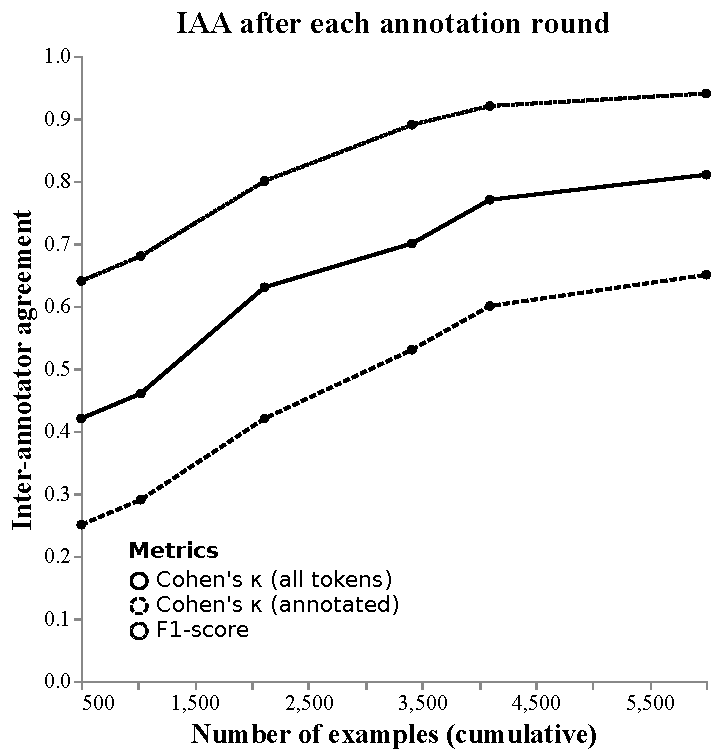
\includegraphics[width=0.5\textwidth]{images/iaa}
\caption{
  Inter-annotator agreement measurement after each annotation round.
  Each mark represents the end of a round. 
  For each round, the annotators discuss disagreements, update the annotation guidelines, and evaluate the current set of annotations.
}
\label{fig:iaa}
\end{figure}

% Entries for the entire Anthology, followed by custom entries
\bibliography{custom}
\bibliographystyle{acl_natbib}


\end{document}
